\section{Modelo de Sistema y Formulación del Problema}

\subsection{3.1. Arquitectura y Modelo de Canal}

Resulta revelador observar cómo la arquitectura NTN integra múltiples capas orbitales con el segmento terrestre de manera mucho más fluida de lo que los estándares iniciales permitían. En este trabajo consideramos una constelación LEO con satélites a 550-1200 km de altitud, equipados con antenas phased-array capaces de beamforming dinámico, enlaces inter-satélite (ISL) y gateways terrestres de alta capacidad.

Aunque los modelos de propagación satelital clásicos proporcionan una base sólida, su aplicación directa en NTN 6G exige ajustes significativos por la movilidad extrema y las condiciones atmosféricas variables. 

\cite{Giuliano2023} ofrece una revisión detallada de arquitecturas y modelos de canal realistas que hemos adoptado como punto de partida. El path loss total se modela combinando pérdida por espacio libre, atenuación atmosférica y efectos de shadowing según recomendaciones ITU-R.

\begin{equation}
PL(d) = FSPL + A_{atm} + A_{shadow} \quad \text{(Eq. 1)}
\end{equation}

donde $FSPL$ representa la free-space path loss dependiente de la distancia slant-range, $A_{atm}$ la atenuación atmosférica y $A_{shadow}$ el shadowing log-normal. La ganancia de antena y el beamforming adaptativo se incorporan mediante patrones de array factor variables en el tiempo.

\begin{figure}[h]
\centering
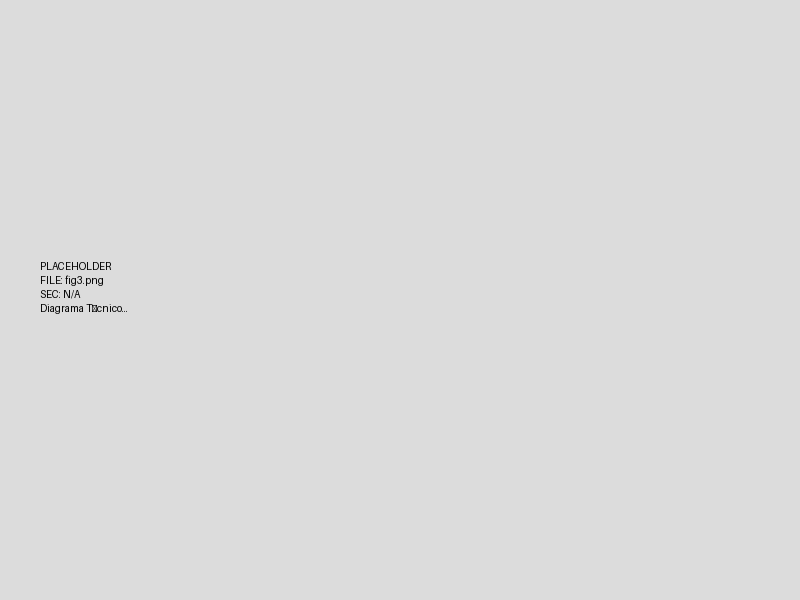
\includegraphics[width=\linewidth]{fig3.png}
\caption{Escenario de simulación NTN con constelación LEO de 6 satélites, distribución heterogénea de usuarios terrestres y beams adaptativos. Se muestran enlaces activos, interferencia co-canal y trayectorias orbitales.}
\label{fig:escenario_simulacion}
\end{figure}

Este modelo captura la dinámica esencial del canal, incluyendo Doppler y variaciones rápidas de ángulo de elevación, elementos críticos que influyen directamente en la viabilidad de cualquier esquema de optimización en tiempo real.

\subsection{3.2. Modelo de Interferencia y Recursos}

Uno de los aspectos más desafiantes al diseñar sistemas NTN radica en el manejo preciso de la interferencia. A diferencia de redes terrestres densas, aquí la interferencia co-canal proviene principalmente de beams adyacentes del mismo satélite o de satélites cercanos en la constelación.

Consideramos un sistema con $N$ satélites y $K$ usuarios terrestres por celda. Cada satélite dispone de recursos limitados: potencia total transmitida $P_{max}$, ancho de banda total $B$ y un número finito de beams. La asignación de recursos se realiza de forma discreta en slots temporales para capturar la dinámica orbital.

Particularmente llamativo es el trade-off inherente entre potencia asignada, ancho de banda y dirección del beam. Asignaciones agresivas de potencia para usuarios lejanos tienden a elevar la interferencia sobre usuarios cercanos en beams vecinos, degradando el rendimiento global del sistema. El modelo de interferencia considera tanto contribuciones intra-satélite como inter-satélite, ponderadas por la ganancia de antena en la dirección del interferidor.

\subsection{3.3. Formulación Matemática del Problema de Optimización}

Lejos de ser un problema de optimización convexo sencillo, la gestión de recursos en NTN bajo movilidad constituye un proceso de decisión secuencial inherentemente estocástico. Formulamos el problema como un Proceso de Decisión de Markov (MDP) multi-agente, donde cada satélite actúa como agente que interactúa con un entorno compartido.

El estado $s_t$ en el instante $t$ incluye información de posiciones relativas, estimaciones de canal, demandas de usuarios y niveles de interferencia actuales. El espacio de acciones $a_t$ abarca la asignación conjunta de potencia, ancho de banda y configuración de beams para los usuarios servidos. 

La función de reward se diseña para balancear múltiples objetivos:

\begin{equation}
r_t = w_1 \cdot R_{sum} - w_2 \cdot I_{agg} + w_3 \cdot J_{fair} - w_4 \cdot P_{out}
\quad \text{(Eq. 2)}
\end{equation}

donde $R_{sum}$ es el throughput sum-rate agregado, $I_{agg}$ la interferencia agregada, $J_{fair}$ el índice de Jain y $P_{out}$ la probabilidad de outage. Los pesos $w_i$ permiten ajustar prioridades según escenarios operativos.

\cite{Ibrahim2026} reporta mejoras sustanciales al emplear guías de Large AI Models en formulaciones MDP similares, aspecto que incorporamos para enriquecer el proceso de aprendizaje y mejorar la convergencia. La tasa instantánea para cada usuario sigue la fórmula Shannon modificada por SINR efectivo:

\begin{equation}
R_k = B_k \log_2(1 + \gamma_k)
\end{equation}

con $\gamma_k$ representando el SINR experimentado por el usuario $k$ tras considerar interferencia y ruido.

Esta formulación captura la complejidad real del problema: espacio de estados y acciones enorme, observabilidad parcial y fuerte acoplamiento entre agentes. Resolverlo mediante métodos tradicionales resulta inviable, justificando plenamente el recurso a técnicas avanzadas de inteligencia artificial que desarrollaremos en la siguiente sección.